%*******************************************************%
%														%
% William Cunningham									%
% wcunning@umich.edu									%
% EECS 470 -- Lab 2										%
%														%
%*******************************************************%

%*******************************************************%
% Preamble												%
%*******************************************************%

\documentclass[dvipsnames]{beamer}
\usetheme{Lab}

\usepackage{
	siunitx,
	tikz,
	graphicx,
	amsmath,
	float,
	minted,
	hyperref,
	textcomp,
	upquote
}

%\usepackage[T1]{fontenc}
%-----------------------%
% TikZ					%
%-----------------------%
%--- CircuiTikZ Definitions ---%

%--- TikZ Definitions ---%
\usetikzlibrary{shapes,arrows,automata,shadows}
\pgfdeclarelayer{background}
\pgfdeclarelayer{foreground}
\pgfsetlayers{background,main,foreground}
% Block Diagram Styles
\tikzstyle{block} = [draw, fill=RoyalBlue!50, rounded corners, rectangle,
        minimum height=2cm, minimum width=2cm]
\tikzstyle{sum} = [draw, fill=blue!20, circle, node distance=2cm]
\tikzstyle{input} = [coordinate]
\tikzstyle{output} = [coordinate]
\tikzstyle{branch} = [coordinate]
\tikzstyle{pinstyle} = [pin edge={to-, thin, black}]
% Signal Flow Graph Styles
\tikzstyle{signal} = [draw, fill=blue!20, circle,
	minimum height=3em]

\definecolor{darkblue}{rgb}{0,0,0.8}

\hypersetup{colorlinks=true,linkcolor=,urlcolor=red}

%*******************************************************%
% Document												%
%*******************************************************%

\title[Lab 3: Style]{EECS 470 Lab 3}
\subtitle{SystemVerilog Style Guide}
\institute[University of Michigan]{Department of Electrical Engineering and 
			Computer Science \\
			College of Engineering \\
			University of Michigan}
\date{Thursday, 19$^\text{th}$ September 2019}

\begin{document}
\frame{\titlepage}

\begin{frame}{Overview}
	\tableofcontents
\end{frame}

\section{Administrivia}
\begin{frame}{Administrivia}
	\begin{block}{Homework}
		\begin{itemize}
			\item Homework 2 is due Thursday, 31$^{\text{st}}$ January at 11:59PM (via Gradescope)
		\end{itemize}
	\end{block}
	\begin{block}{Projects}
		\begin{itemize}
			\item Project 2 is due Monday, 23$^{\text{th}}$ September
				at 11:59PM (via submission script)
		\end{itemize}
	\end{block}
	\begin{block}{Help}
		We are available to answer questions on anything here. Office hours can
		be found on the
		\href{https://www.eecs.umich.edu/courses/eecs470/}{course
		web site}.
	\end{block}
\end{frame}

\section{Verilog Style Guide}
\begin{frame}{Verilog Style}
	\begin{block}{What is good style?}
		\begin{itemize}
			\item Easy to read
			\item Easy to understand
			\item Mostly a matter of personal preference
		\end{itemize}
	\end{block}
	\begin{block}{Why should I use good style?}
		\begin{itemize}
			\item Easier to debug
			\item Important for group work
			\item Mandatory in projects 1-3
		\end{itemize}
	\end{block}
\end{frame}


\begin{frame}{Verilog Style Rules}
	\begin{block}{Goal: Clarity}
		\begin{itemize}
			\item For any problem, one solution is the clearest
			\item We want to approximate this solution
			\item By creating a set of rules to follow
		\end{itemize}
	\end{block}
	\begin{block}{Format}
		\begin{itemize}
			\item We'll look at a bad example
			\item Then how to fix it
			\item Derive a rule
		\end{itemize}
	\end{block}
\end{frame}

\subsection{Brevity}

\begin{frame}[fragile]{Brevity by Example}
\begin{columns}
	\begin{column}[T]{0.45\textwidth}
		\begin{block}{Example}
		\begin{minted}[tabsize=4, fontsize=\scriptsize]{verilog}
always_comb
begin
    if (foo[3] == 1'b1)
    begin
        bar[3] = 1'b1;
        bar[2] = 1'b0;
        bar[1] = 1'b1;
        bar[0] = 1'b1;
    end else if (foo[2] == 1'b1)
    begin
        bar[3] = 1'b0;
        bar[2] = 1'b1;
        bar[1] = 1'b0;
        bar[0] = 1'b0;
    end
end
		\end{minted}
		\end{block}
	\end{column}
	\pause
	\begin{column}[T]{0.1\textwidth}
		\vspace*{0.25\textheight}
		\large{vs.}
		\normalsize
	\end{column}
	\begin{column}[T]{0.45\textwidth}
		\begin{block}{Example Reformatted}
		\begin{minted}[tabsize=4, fontsize=\scriptsize]{verilog}
always_comb
begin
    if (foo[3])      bar = 4'b1011;
    else if (foo[2]) bar = 4'b0100;
end
		\end{minted}
		\end{block}
	\end{column}
\end{columns}
\end{frame}

\begin{frame}[fragile]{Brevity by Example}
\begin{columns}
	\begin{column}[T]{0.45\textwidth}
		\begin{block}{Example}
		\begin{minted}[tabsize=4, fontsize=\scriptsize]{verilog}
logic [5:0] shift;

always_ff @(posedge clock)
begin
    if (reset)
    begin
        shif_reg <= #1 6'b0;
    end else begin
        shift[0] <= #1 foo;
        shift[1] <= #1 shift[0];
        shift[2] <= #1 shift[1];
        shift[3] <= #1 shift[2];
        shift[4] <= #1 shift[3];
        shift[5] <= #1 shift[4];
    end
end
		\end{minted}
		\end{block}
	\end{column}
	\pause
	\hspace*{-24pt}
	\begin{column}[T]{0.05\textwidth}
		\vspace*{0.25\textheight}
		\large{vs.}
		\normalsize
	\end{column}
	\begin{column}[T]{0.475\textwidth}
		\begin{block}{Example Reformatted}
		\begin{minted}[tabsize=4, fontsize=\scriptsize]{verilog}
logic [5:0] shift;

always_ff @(posedge clock)
begin
    if (reset) 
    begin
        shift <= #1 6'b0;
    end else begin
        shift <= #1 {shift[4:0], foo};
    end
end
		\end{minted}
		\end{block}
	\end{column}
\end{columns}
\end{frame}

\begin{frame}{Brevity Rule}
	\begin{block}{Rule}
		Brevity is strongly correlated with the optimal solution. Be brief,
		where you can.	
	\end{block}
\end{frame}

\begin{frame}{General Requirements}
	\begin{block}{Clarity Rules}
		\begin{itemize}
			\item Use meaningful names for signal; \texttt{wire wire;} is
				confusing
			\item Comment your designs; \texttt{(a \^{} b \~{}\^{} c) | (\&d)}
				is unintelligible without an explanation
			\item Conceptualize what you need to build before you start writing
				Verilog. A state machine diagram will be make the Verilog much
				easier\dots
		\end{itemize}
	\end{block}
\end{frame}

\subsection{Indentation and Alignment}

\begin{frame}{Indentation}
	\begin{block}{Why are we interested in indentation?}
		\begin{itemize}
			\item Readability -- easier to trace down
			\item Clarity -- easier to check what is in a given scope
		\end{itemize}
	\end{block}
\end{frame}

\begin{frame}[fragile]{Indentation by Example}
	\begin{columns}
		\begin{column}[T]{0.35\textwidth}
			\begin{block}{Example}
				\vspace*{0pt}
				\begin{minted}[tabsize=4, fontsize=\scriptsize,]{verilog}
always_comb 
begin
if(cond) 
begin
n_state = `IDLE;
n_gnt = `NONE;
end else begin
n_state = `TO_A;
n_gnt = `GNT_A;
end
end
				\end{minted}
			\end{block}
		\end{column}
		\pause
		\begin{column}[T]{0.05\textwidth}
			\vspace*{0.3\textheight}
			\large{vs.}
			\normalsize
		\end{column}
		\begin{column}[T]{0.35\textwidth}
			\begin{block}{Example Reformatted}
				\vspace*{0pt}
				\begin{minted}[tabsize=4, fontsize=\scriptsize,]{verilog}
always_comb
begin
    if (cond)
    begin
        n_state = `IDLE;
        n_gnt = `NONE;
    end else begin
        n_state = `TO_A;
        n_gnt = `GNT_A;
    end
end
				\end{minted}
			\end{block}
		\end{column}
	\end{columns}
\end{frame}

\begin{frame}{Indentation Rule}
	\begin{block}{Rule}
		Items within the same scope should have the same indentation.
	\end{block}
\end{frame}

\begin{frame}{Alignment}
	\begin{block}{Why are we interested in alignment?}
		\begin{itemize}
			\item Readability -- easier to trace down
			\item Clarity -- easier to check that everything is assigned
		\end{itemize}
	\end{block}
\end{frame}

\begin{frame}[fragile]{Alignment by Example}
	\begin{columns}
		\begin{column}[T]{0.35\textwidth}
		\begin{block}{Example}
			\vspace*{0pt}
			\begin{minted}[tabsize=4, fontsize=\scriptsize,]{verilog}
always_comb
begin
    if (cond)
    begin
        n_state = `IDLE;
        n_gnt = `NONE;
    end else begin
        n_state = `TO_A;
        n_gnt = `GNT_A;
    end
end
			\end{minted}
		\end{block}
		\end{column}
		\pause
		\begin{column}[T]{0.1\textwidth}
			\vspace*{0.3\textheight}
			\large{vs.}
			\normalsize
		\end{column}
		\begin{column}[T]{0.35\textwidth}
		\begin{block}{Example Reformatted}
			\vspace*{0pt}
			\begin{minted}[tabsize=4, fontsize=\scriptsize,]{verilog}
always_comb
begin
    if (cond)
    begin
        n_state  = `IDLE;
        n_gnt    = `NONE;
    end else begin
        n_state  = `TO_A;
        n_gnt    = `GNT_A;
    end
end
			\end{minted}
		\end{block}
		\end{column}
	\end{columns}
\end{frame}

\begin{frame}[fragile]{Alignment by Example}
	\begin{block}{Example}
		\begin{minted}[tabsize=4, fontsize=\scriptsize,frame=lines]{verilog}
assign mux_out = (cond1) ? (foo1&bar): (cond2) ? (foo2+cnt3) :
(cond3) ? (foo3&~bar2) : 0;
		\end{minted}
	\end{block}
	\pause
	\begin{block}{Example Reformatted}
		\begin{minted}[tabsize=4, fontsize=\scriptsize,frame=lines]{verilog}
assign mux_out = (cond1) ? (foo1 & bar) :
                 (cond2) ? (foo2 + cnt3) :
                 (cond3) ? (foo3 & ~bar2) : 0;
		\end{minted}
	\end{block}
\end{frame}

\begin{frame}{Alignment Rule}
	\begin{block}{Rule}
		Assignments should be aligned by column. \\
		Ternary statements should have the conditionals aligned, and each ``if''
		should be on a new line.
	\end{block}
\end{frame}


\subsection{SystemVerilog Features}

\begin{frame}{SystemVerilog Types}
	\begin{block}{User-defined Types}
		\begin{itemize}
			\item Useful for cleaning repeated declarations, specifically
				bundling connections
			\item Types can be named informatively, e.g. \texttt{arch\_reg\_t}
		\end{itemize}
	\end{block}
\end{frame}

\begin{frame}{Structs}
	\begin{block}{About \texttt{struct}}
		\begin{itemize}
			\item A package of signals (\texttt{wire} or \texttt{logic})
			\item Basically follow C conventions
				\begin{itemize}
					\item List of signal declarations
					\item Named with \texttt{\_t} ending
				\end{itemize}
		\end{itemize}
	\end{block}
	\begin{block}{Syntax}
		\begin{itemize}
			\item \texttt{struct}
			\item List of signals between braces (\texttt{\{\}})
			\item Name after braces, followed by a semicolon (\texttt{;})
		\end{itemize}
	\end{block}
\end{frame}

\begin{frame}[fragile]{Structs}
	\begin{block}{Example}
		\vspace*{-12pt}
		\begin{minted}[frame=lines,fontsize=\scriptsize]{systemverilog}
			typedef struct {
			    logic [7:0] a; //Structs can contain
			    logic       b; //other structs, like
			    arch_reg_t  c; //<-- this line
			} example_t; //named with _t
		\end{minted}
	\end{block}
	\begin{block}{Example}
		\vspace*{-12pt}
		\begin{minted}[frame=lines,fontsize=\scriptsize]{systemverilog}
			typedef struct packed {
			    addr_t  pc;
			    logic   valid;
			} prf_entry_t;
		\end{minted}
	\end{block}
	\begin{block}{Usage Example}
		\vspace*{-12pt}
		\begin{minted}[frame=lines,fontsize=\scriptsize]{systemverilog}
			prf_entry_t [31:0] prf;
			assign prf[1].valid = 1'b0;
		\end{minted}
	\end{block}
\end{frame}

\begin{frame}{Enums}
	\begin{block}{About \texttt{enum}}
		\begin{itemize}
			\item List of possible values, but named instead of numbered
			\item Good for state machine states
			\item Can be shown in DVE instead of the associated value
		\end{itemize}
	\end{block}
	\begin{block}{Syntax}
		\begin{itemize}
			\item \texttt{enum}
			\item List of values between braces (\texttt{\{\}})
			\item Name after braces, followed by a semicolon (\texttt{;})
		\end{itemize}
	\end{block}
\end{frame}

\begin{frame}[fragile]{Enums}
	\vspace*{-12pt}
	\begin{block}{Example}
		\vspace*{-12pt}
		\begin{minted}[frame=lines,fontsize=\scriptsize]{systemverilog}
			typedef enum logic [3:0] {
			    IDLE,     //=0, by default
			    GNT[0:7], //Expands to GNT0=1,...GNT7=8
			    RESET     //=9
			} arb_state;
		\end{minted}
	\end{block}
	\begin{block}{Example}
		\vspace*{-12pt}
		\begin{minted}[frame=lines,fontsize=\scriptsize]{systemverilog}
			typedef enum logic [1:0] {
			    ADD   = 2'b00,  //The value associated with
			    MULT  = 2'b10,  //a particular name can be
			    NOT   = 2'b11,  //assigned explicitly.
			    AND   = 2'b01
			} opcode;
		\end{minted}
	\end{block}
	\begin{block}{Usage Example}
		\vspace*{-12pt}
		\begin{minted}[frame=lines,fontsize=\scriptsize]{systemverilog}
			arb_state state, n_state;
			assign n_state = IDLE;
		\end{minted}
	\end{block}
\end{frame}

\begin{frame}{Enums}
	\begin{block}{DVE Example}
		\begin{figure}[h]
			\centering
			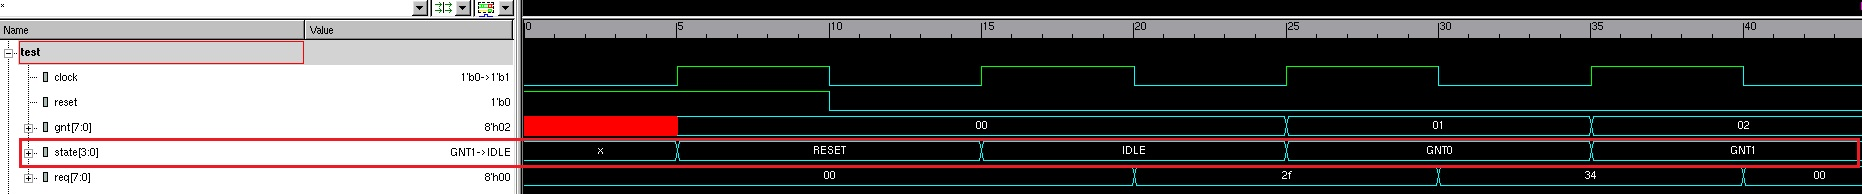
\includegraphics[width=1\textwidth,clip,trim=0 0 10cm 0]{enum_dve.jpg}
		\end{figure}
	\end{block}
\end{frame}

\begin{frame}[fragile]{Typedef}
	\begin{block}{About \texttt{typedef}}
		\begin{itemize}
			\item Necessary for reuse of a \texttt{struct} or \texttt{enum}
				\begin{itemize}
					\item Without a \texttt{typedef}, a
						\texttt{struct}/\texttt{enum} must be redefined
						at each instance declaration
				\end{itemize}
			\item Also useful in clearly naming commonly sized buses
		\end{itemize}
	\end{block}
	\begin{block}{Syntax}
		\begin{itemize}
			\item \texttt{typedef}
			\item by any signal declaration or \texttt{struct} or \texttt{enum}
				declaration
			\item Name for the type followed by a semicolon (\texttt{;})
		\end{itemize}
	\end{block}
\end{frame}

\begin{frame}[fragile]{Typedef by Example}
	\begin{block}{Example: Typedef'd Enum}
		\vspace*{-12pt}
		\begin{minted}[frame=lines,fontsize=\scriptsize]{systemverilog}
			//typedef, then definition, then name;
			typedef enum logic [3:0] {
			    IDLE,     
			    GNT[0:7], 
			    RESET     
			} arb_state;
		\end{minted}
	\end{block}
	\begin{block}{Example: Type Synonym}
		\vspace*{-12pt}
		\begin{minted}[frame=lines,fontsize=\scriptsize]{systemverilog}
			//typedef, then definition, then name;
			typedef logic [63:0] addr;
		\end{minted}
	\end{block}
\end{frame}

\section{Finite State Machines}
\begin{frame}{Procedural FSM Design}
	\begin{block}{FSM Process}
		\begin{itemize}
			\item All states should be \texttt{typedef enum}
			\item All next state logic should go into a combinational block,
				following all combinational rules
			\item All resets should be synchronous (to the clock)
			\item All output assignments should go in their own combinational
				block
			\item The only logic in the sequential block should be the state
				assignment (to the computed next state)
		\end{itemize}
	\end{block}
\end{frame}

\begin{frame}[fragile]{Finite State Machine Skeleton}
	\vspace*{-12pt}
	\begin{minted}[tabsize=4, frame=lines,fontsize=\scriptsize,mathescape]{systemverilog}
typedef enum logic [(NUM_STATES-1):0] { STATES } fsm_state;

module fsm(
    input wire inputs,
    output logic outputs
    );

    fsm_state state, next_state;

    always_comb begin
    /* Transitions from a diagram go here */
    /* $\mathtt{next\_state} = f(\mathtt{inputs},\mathtt{state})$ */
    end

    always_ff @(posedge clock) begin
        if(reset) begin
            state <= #1 DEFAULT;
        end else begin
            state <= #1 next_state;
        end
    end
endmodule
	\end{minted}
\end{frame}

\begin{frame}{Finite State Machine Example}
	\vspace*{-12pt}
	\inputminted[frame=lines,fontsize=\scriptsize,tabsize=4,obeytabs=true]{systemverilog}{verilog/fsm.v}
\end{frame}
\begin{frame}{Coverage}
    \begin{itemize}
        \item So last time we talked about why to write a testbench
        \item We also talked about how to write a good testbench
        \item All metrics that we talked about are rather qualitative, though
        \item How do we quantitatively measure how good a testbench is - code coverage
    \end{itemize}
\end{frame}

\begin{frame}{Coverage Cont.}
    \begin{block}{Code Coverage Types}
        \begin{itemize}
            \item Line Coverage — This metric measures statements in your HDL code that have been executed in the simulation
            \item Toggle Coverage — This metric measures the bits of logic that have toggled during simulation. A toggle simply means that a bit changes from 0 to 1 or from 1 to 0. It is one of the oldest metrics of coverage in hardware designs and can be used at both the register transfer level (RTL) and gate level.
            \item Condition Coverage — This metric measures how the variables or sub-expressions in the conditional statements are evaluated during simulation. It can find errors in the conditional statements that cannot be found by other coverage analysis.
        \end{itemize}
    \end{block}
\end{frame}
\begin{frame}{Coverage Cont.}
    \begin{block}{Code Coverage Types Cont.}
        \begin{itemize}
            \item Branch Coverage — This metric measures the coverage of expressions and case statements that affect the control flow (such as if-statement and while-statement) of the HDL. It focuses on the decision points that affect the control flow of the HDL execution.
            \item FSM Coverage — This metric verifies that every legal state of the state machine has been visited and that every transition between states has been covered.
            \item For more information about coverage, feel free to ask us or search online!
        \end{itemize}
    \end{block}
\end{frame}
\begin{frame}{Coverage Cont.}
    \begin{block}{Coverage compile time options}
        \begin{itemize}
        
            \item \texttt{-cm line|cond|fsm|tgl|branch|assert}
            \item The arguments specifies the types of coverage:
                \begin{itemize}
                    \item \texttt{line   Compile for line or statement coverage.}
                    \item \texttt{cond   Compile for condition coverage.}
                    \item \texttt{fsm    Compile for FSM coverage.}
                    \item \texttt{tgl    Compile for toggle coverage.}
                    \item \texttt{branch Compile for branch coverage}
                    \item \texttt{assert Compile for SystemVerilog assertion coverage.}
                \end{itemize}
             \item If you want VCS to compile for more than one type of coverage, use the plus (+) character as a delimiter between arguments, for example:
                \begin{itemize}
                    \item \texttt{-cm line+cond+fsm+tgl}
                \end{itemize}
        \end{itemize}
    \end{block}
\end{frame}
\begin{frame}{Coverage example}
    \texttt{vcs -V -sverilog +vc -Mupdate -line -full64 +vcs+vcdpluson -debug\_{pp} -cm line+tgl mydesign.v mytest.v -o simv}
    
    \texttt{./simv -cm line+tgl}
    
    \texttt{urg -dir simv.vdb -format text}
    \\
    \\
    Note: To use \texttt{urg}, you need to run the following command in the terminal:
    \\
    \\
    \texttt{module load vcs} 
    \\
    \\
    you should then see a generated directory named \texttt{urgReport} and within it you'll find a \texttt{hierarchy.txt}
    it should have something like:
\end{frame}

\begin{frame}{Coverage example Cont.}
	\inputminted[frame=lines,fontsize=\scriptsize,tabsize=4,obeytabs=true]{text}{hierarchy.txt}
\end{frame}

\begin{frame}{Coverage Cont.}
    We will come back to this later in the final project.
    As part of milestone 1, you will need to submit a module along with a testbench and we will grade you based on your coverage percentage, but that'll be much later.
    In the meanwhile... Give it a try on your project 2 testbench!
\end{frame}

\section{Project 2}
\begin{frame}{Project 2 Overview}
	\begin{block}{Part 1: Pipelined Multiplier}
		\begin{itemize}
			\item Change the pipeline depth
			\item Synthesize at each size
		\end{itemize}
	\end{block}
	\begin{block}{Part 2: Integer Square Root}
		\begin{itemize}
			\item Finite state machine implementation
			\item Synthesis
		\end{itemize}
	\end{block}
\end{frame}

\begin{frame}{Pipelined Multiplication}
	\begin{block}{Partial Products}
		\begin{itemize}
			\item Multiply the first $n$ bits of the two components
			\item Multiply the next $n$ bits, etc.
			\item Sum the partial products to get the answer
		\end{itemize}
	\end{block}
\end{frame}

\begin{frame}{Pipelined Multiplication by Example}
	\setlength{\tabcolsep}{2pt}
	\begin{columns}
		\begin{column}[T]{0.45\textwidth}
			\begin{block}{Binary Multiplication}
				\begin{tabular}{cccccccc}
								& 0 & 0 & 0 & 1 & 1 & 1 \\
					$\times$	&   &   & 0 & 1 & 0 & 1 \\ \hline
								& 0 & 0 & 0 & 1 & 1 & 1 \\
								& 0 & 0 & 0 & 0 & 0 & 0 \\
								& 0 & 1 & 1 & 1 & 0 & 0 \\
						+		& 0 & 0 & 0 & 0 & 0 & 0 \\ \hline
								& 1 & 0 & 0 & 0 & 1 & 1 
				\end{tabular}
			\end{block}
		\end{column}
		\begin{column}[T]{0.45\textwidth}
			\begin{block}{Decimal Multiplication}
				\begin{tabular}{ccc}
								&   & 7 \\
					$\times$	&   & 5 \\ \hline
								& 3 & 5
				\end{tabular}
			\end{block}
		\end{column}
	\end{columns}
\end{frame}

\begin{frame}{Pipelined Multiplication by Example}
	\begin{block}{Example: 4-stage Pipelined Multiplication}
		\begin{tabular}{rll}
			multiplicand:
				& 
				\only<1>{00001011} 
				\only<2>{\hspace*{0pt}00001011} 
				\only<3>{\hspace*{0pt}00101100} 
				\only<4>{\hspace*{0pt}00101100} 
				&
				\only<2>{\alert{\texttt{<{}< 2}}}
				\only<4>{\alert{\texttt{<{}< 2}}}
				\\
			multiplier:
				& 
				\only<1>{000001\alert{11}}
				\only<2>{00000111}
				\only<3>{000000\alert{01}}
				\only<4>{00000001}
				&
				\only<2>{\alert{\texttt{>{}> 2}}}
				\only<4>{\alert{\texttt{>{}> 2}}}
				\\
			partial product:
				& 
				\only<1>{\texttt{00000000}}
				\only<2>{\alert{\texttt{00100001}}}
				\only<3>{\texttt{00100001}}
				\only<4>{\alert{\texttt{01001101}}}
		\end{tabular}
		
		\vspace*{24pt}
		
		\setlength{\tabcolsep}{2pt}
		\begin{onlyenv}<1-2>
			\begin{tabular}{ccccccccc}
							& 0 & 0 & 0 & 0 & 1 & 0 & 1 & 1 \\
				$\times$	& 0 & 0 & 0 & 0 & 0 & 0 & \alert<1>{1} &
				\alert<1>{1} \\ \hline
							& 0 & 0 & \temporal<2>{0}{1}{} & 0 & 0 & 0 & 
							0 & \temporal<2>{0}{1}{} \\
			\end{tabular}
		\end{onlyenv}
		\begin{onlyenv}<3-4>
			\begin{tabular}{ccccccccc}
							& 0 & 0 & 1 & 0 & 1 & 1 & 0 & 0 \\
				$\times$	& 0 & 0 & 0 & 0 & 0 & 0 & \alert<3>{0} &
				\alert<3>{1} \\ \hline
				& 0 & 0 & \temporal<4>{0}{1}{} & 0 &
				\temporal<4>{0}{1}{} & \temporal<4>{0}{1}{} & 0 & 0 \\
			\end{tabular}
		\end{onlyenv}
	\end{block}
\end{frame}

\begin{frame}{Part 1 Hints}
	\begin{block}{Pipeline Depth}
		\begin{itemize}
			\item Figure out the sizes of all the structures as a function 
				of pipeline depth
			\item This would be an optimal place to use \texttt{\`{}define}
		\end{itemize}
	\end{block}
	\begin{block}{Synthesis}
		\begin{itemize}
			\item Clock Periods ($T_{clk}$)
				\begin{itemize}
					\item Optimize inner module (\texttt{mult\_stage.v}) first,
						then outer (\texttt{mult.v})
					\item Understand \texttt{set\_dont\_touch}
				\end{itemize}
			\item Synthesis is time consuming; $\approx$ 10 minutes for both
				\texttt{mult\_stage} and \texttt{mult}
		\end{itemize}
	\end{block}
\end{frame}

\begin{frame}{Part 2 Hints}
	\begin{block}{ISR Algorithm}
		\begin{itemize}
			\item Guess-and-check
			\item Loop from the top bit of the guess to the bottom
			\item Basically binary search for a solution
		\end{itemize}
	\end{block}
	\begin{block}{Hardware Implementation}
		\begin{itemize}
			\item How do we implement this in hardware?
		\end{itemize}
	\end{block}
\end{frame}

\begin{frame}{Part 2 Hints}
	\begin{block}{ISR State Machine}
		Computing: $\sqrt{\mathtt{value}}$
		\begin{itemize}
			\item On a \texttt{reset}
				\begin{itemize}
					\item \texttt{guess} initialized to \texttt{32'h8000\_0000}	
					\item \texttt{value} is clocked into a register
				\end{itemize}
			\item \texttt{guess} gets the next bit set each time we cycle
				through the FSM again
			\item Square \texttt{guess} (multiply it with itself)
				\begin{itemize}
					\item Wait until the multiplier raises its \texttt{done}
				\end{itemize}
			\item if \texttt{guess <= value} 
				\begin{itemize}
					\item Keep the current bit
				\end{itemize}
			\item else 
				\begin{itemize}
					\item Clear the current bit
				\end{itemize}
			\item Move to the next bit
			\item After the last bit, raise \texttt{done}
		\end{itemize}
	\end{block}
\end{frame}

\begin{frame}{Part 2 Hints}
	\begin{block}{Reminders}
		\begin{itemize}
			\item Remember to declare bitwidths for signals, e.g.
				\texttt{64'hFFFF\_FFFF\_FFFF\_FFFF}
			\item It must take less than 600 cycles to compute a square root
			\item Remember to use the 8-stage multiplier for this
			\item Remember to check for proper reset behavior
			\item Remember the reset pragma (\texttt{//synopsys sync\_set\_reset
				``reset''})
		\end{itemize}
	\end{block}
\end{frame}

\begin{frame}{Lab Assignment}
	\begin{itemize}
		\item Assignment is posted to the \href{http://www.eecs.umich.edu/eecs/courses/eecs470}{\underline{course website}} as Lab
			3 Assignment.
		\item If you get stuck\dots
			\begin{itemize}
				\item Ask a neighbor, quietly
				\item Put yourself in the 
					\href{https://oh.eecs.umich.edu/courses/eecs470}{\underline{help queue}}
			\end{itemize}
		\item When you are finished, put yourself on help queue to get checked off.
		\item If you are unable to finish today, the assignment needs to be
			checked off by next Thursday.
	\end{itemize}
\end{frame}
\end{document}

